
% \titlegraphic{\hfill\includegraphics[height=1.5cm]{logo.pdf}}

\documentclass[xcolor=pdftex,dvipsnames,table,numbers,hyperref={pdfpagelabels=false},compress]{beamer}
%\usepackage{requiredPackage}
\usepackage{amsmath}
\usepackage{graphicx}
\usepackage{amsfonts}
\usepackage{amssymb}

\usepackage{tabularx}
\usepackage{epstopdf}
\usepackage{overpic}
\usepackage{url}
\usepackage{calrsfs}
\usepackage{mathrsfs}
\usepackage{epsfig}
\usepackage{cancel}
\usepackage{changepage}

\usepackage{tikz}
\usepackage[customcolors]{hf-tikz} 

\usepackage{lmodern}
%\usepackage{mystyle}
\usepackage{subfig}
\usepackage{pifont}
\usepackage{tabu}
\usepackage{xcolor}
\usepackage{algorithm}
\usepackage{algpseudocode}
%\usepackage{enumitem}
\usepackage{remreset}
\usepackage{etoolbox}
\usepackage{comment} % end and begin comment
%\usepackage{dtklogos} 
\usepackage{listings}
\lstset{breaklines=true} 

\newcommand{\gline}{\textcolor{gray}{\hline}}
\newcommand{\cmark}{\ding{51}}%
\newcommand{\xmark}{\ding{55}}%
\newcommand{\gcheck}{\textcolor{blue}{\Large \cmark}}
\newcommand{\rcross}{\textcolor{red}{\Large \xmark}}
\newcommand{\tkt}{\tilde{K}_\theta}
\newcommand{\kt}{K_\theta}
\newcommand{\ind}{\overset{ind}{\sim}}
\newcommand{\plim}{\overset{p}{\rightarrow}}
\newcommand{\cx}{\frac {X'X}n}
\newcommand{\cz}{\frac {Z'Z}n}
\newcommand{\ccz}{\frac {Z'Z}n - \Sigma_A}
\newcommand{\czy}{\frac {Z'y}n}
\newcommand{\cyz}{\frac {y'Z}n}
\newcommand{\cxy}{\frac {X'y}n}
\newcommand{\cyx}{\frac {y'X}n}
\newcommand{\myitem}{\vskip3mm \item}

\newcommand{\calS}{{\cal S}}
\newcommand{\calA}{{\cal A}}
\newcommand{\calK}{{\cal K}}
\newcommand{\calX}{{\cal X}}
\newcommand{\calD}{{\cal D}}
\newcommand{\calG}{{\cal G}}
\newcommand{\calT}{{\cal T}}
\newcommand{\calU}{{\cal U}}
\newcommand{\calR}{{\cal R}}
\newcommand{\tp}{\tilde{p}}
\newcommand{\tildebC}{\tilde{\bC}}
\newcommand{\calL}{{\cal L}}

\newcommand{\blam}{ \mbox{\boldmath $ \lambda $} }
\newcommand{\bet}{ \mbox{\boldmath $ \eta $} }
\newcommand{\bome}{ \mbox{\boldmath $ \omega $} }
\newcommand{\bbet}{ \mbox{\boldmath $ \beta $} }
\newcommand{\bbeta}{ \mbox{\boldmath $ \beta $} }
\newcommand{\balph}{ \mbox{\boldmath $ \alpha $} }
\newcommand{\balpha}{ \mbox{\boldmath $ \alpha $} }
\newcommand{\bphi}{ \mbox{\boldmath $\phi$}}
\newcommand{\bzeta}{ \mbox{\boldmath $\zeta$}}
\newcommand{\bkap}{ \mbox{\boldmath $\kappa$}}
\newcommand{\bkappa}{ \mbox{\boldmath $\kappa$}}
\newcommand{\beps}{ \mbox{\boldmath $\epsilon$}}
\newcommand{\bepsilon}{ \mbox{\boldmath $\epsilon$}}
\newcommand{\bthet}{ \mbox{\boldmath $ \theta $} }
\newcommand{\btheta}{ \mbox{\boldmath $ \theta $} }
\newcommand{\blambda}{ \mbox{\boldmath $ \lambda $} }
\newcommand{\bnu}{ \mbox{\boldmath $\nu$} }
\newcommand{\bmu}{ \mbox{\boldmath $\mu$} }
\newcommand{\bGam}{ \mbox{\boldmath $\Gamma$} }
\newcommand{\bSig}{ \mbox{\boldmath $\Sigma$} }
\newcommand{\bSigma}{ \mbox{\boldmath $\Sigma$} }
\newcommand{\bPhi}{ \mbox{\boldmath $\Phi$} }
\newcommand{\bThet}{ \mbox{\boldmath $\Theta$} }
\newcommand{\bTheta}{ \mbox{\boldmath $\Theta$} }
\newcommand{\bDel}{ \mbox{\boldmath $\Delta$} }
\newcommand{\bDelta}{ \mbox{\boldmath $\Delta$} }
\newcommand{\bnabla}{ \mbox{\boldmath $\nabla$} }
\newcommand{\bLam}{ \mbox{\boldmath $\Lambda$} }
\newcommand{\bLambda}{ \mbox{\boldmath $\Lambda$} }
\newcommand{\bgam}{ \mbox{\boldmath $\gamma$} }
\newcommand{\bgamma}{ \mbox{\boldmath $\gamma$} }
\newcommand{\brho}{ \mbox{\boldmath $\rho$} }
\newcommand{\bdel}{ \mbox{\boldmath $\delta$} }
\newcommand{\bdelta}{ \mbox{\boldmath $\delta$} }
\newcommand{\sis}{\sigma^2}
\newcommand{\bOmega}{\mbox{\boldmath $\Omega$} }
\newcommand{\bPsi}{ {\boldsymbol \Psi} }
\newcommand{\btkt}{\boldsymbol{\tilde{K}}_\theta}
\newcommand{\pg}{P{\'o}lya-Gamma }

\newcommand{\bzero}{\textbf{0}}
\newcommand{\bones}{\textbf{1}}
\newcommand{\ba}{\textbf{a}}
\newcommand{\bb}{\textbf{b}}
\newcommand{\bB}{\textbf{B}}
%\newcommand{\bA}{\textbf{A}}
\newcommand{\bc}{\textbf{c}}
\newcommand{\bC}{\textbf{C}}
\newcommand{\bA}{\textbf{A}}
\newcommand{\bd}{\textbf{d}}
\newcommand{\bD}{\textbf{D}}
\newcommand{\be}{\textbf{e}}
\newcommand{\bE}{\textbf{E}}
\newcommand{\bk}{\textbf{k}}
\newcommand{\bK}{\textbf{K}}
\newcommand{\bh}{\textbf{h}}
\newcommand{\bs}{\textbf{s}}
\newcommand{\bS}{\textbf{S}}
\newcommand{\bH}{\textbf{H}}
\newcommand{\bI}{\textbf{I}}
\newcommand{\bt}{\textbf{t}}
\newcommand{\bu}{\textbf{u}}
\newcommand{\bv}{\textbf{v}}
\newcommand{\bw}{\textbf{w}}
\newcommand{\bW}{\textbf{W}}
\newcommand{\bx}{\textbf{x}}
\newcommand{\bX}{\textbf{X}}
\newcommand{\by}{\textbf{y}}
\newcommand{\bY}{\textbf{Y}}
\newcommand{\bz}{\textbf{z}}
\newcommand{\bZ}{\textbf{Z}}
\newcommand{\bL}{\textbf{L}}
\newcommand{\br}{\textbf{r}}
\newcommand{\bR}{\textbf{R}}
\newcommand{\bm}{\textbf{m}}
\newcommand{\bM}{\textbf{M}}
\newcommand{\given}{\,|\,}
\newcommand{\T}{\top}
\newcommand{\bV}{\textbf{V}}
\newcommand{\bJ}{\textbf{J}}
\newcommand{\blue}[1]{{\color{RoyalBlue!90} #1}}
\newcommand{\red}[1]{{\color{Red} #1}}
\newcommand{\green}[1]{{\color{Green} #1}}
\newcommand{\orange}[1]{{\color{Orange} #1}}
\newcommand{\titl}[1]{{\begin{large}\begin{center}#1\end{center}\end{large}}}

\newcommand{\tildea}{\tilde{a}}
\newcommand{\tildeba}{\tilde{\ba}}
\newcommand{\tildebv}{\tilde{\bv}}
\newcommand{\tildev}{\tilde{v}}
\newcommand{\tildeA}{\tilde{A}}
\newcommand{\tildeC}{\tilde{C}}
\newcommand{\tildeK}{\tilde{K}}
\newcommand{\tildew}{\tilde{w}}
\newcommand{\tildeu}{\tilde{u}}
\newcommand{\tildebw}{\tilde{\bw}}
\newcommand{\tildeeps}{\tilde{\epsilon}}
\newcommand{\tildebeps}{\tilde{\bepsilon}}
\newcommand{\eps}{\epsilon}
\newcommand{\sigs}{\sigma^2}
\newcommand{\taus}{\tau^2}
\newcommand{\iid}{\stackrel{\mathrm{iid}}{\sim}}

%\newcommand{\calS}{{\cal S}}
\newcommand{\calC}{{\cal C}}

%\documentclass[10pt]{beamer}

\usetheme{metropolis}
\usepackage{appendixnumberbeamer}

\usepackage{booktabs}
\usepackage[scale=2]{ccicons}

\usepackage{pgfplots}
\usepgfplotslibrary{dateplot}

\usepackage{xspace}
\newcommand{\themename}{\textbf{\textsc{metropolis}}\xspace}

\makeatletter
\@addtoreset{subfigure}{framenumber}% subfigure counter resets every frame
\makeatother

\makeatletter
\@addtoreset{figure}{framenumber}% subfigure counter resets every frame
\makeatother

\setbeamertemplate{caption}{\raggedright\insertcaption\par}
\captionsetup[subfigure]{labelformat=empty}


\title[]{Nearest Neighbor Gaussian Processes for Large Spatial Data}
\author{Andrew Finley$^1$ \& Jeffrey Doser$^2$}
	
\institute{
\begin{tiny}$^1$Department of Forestry, Michigan State University.\\
$^2$Department of Integrative Biology, Michigan State University.\end{tiny}
}

\date{May 15, 2023}


\begin{document}

\maketitle

\begin{frame}{Low rank Gaussian Predictive Process}
	\only<1>{\begin{alertblock}{Pros}
	\begin{itemize}
		\item Proper Gaussian process
		\item Allows for coherent spatial interpolation at arbitrary resolution
		\item Can be used as prior for spatial random effects in any hierarchical setup for spatial data
		\item Computationally tractable
	\end{itemize}
	\end{alertblock}
	}
	\only<2>{
				\begin{alertblock}{Cons}
					\begin{figure}[t]
				\begin{center}
					\vskip -5mm \subfloat[True $w$]{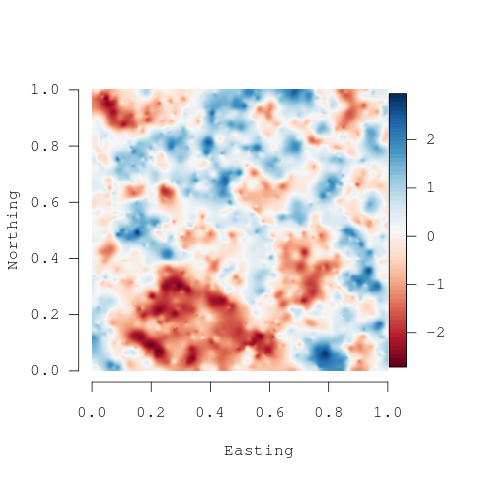
\includegraphics[width=3.5cm]{../figures/w-obs.png}\label{uni-w-obs}}
					\subfloat[Full GP]{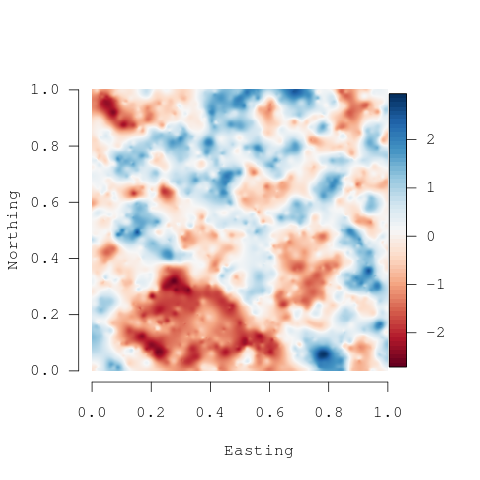
\includegraphics[width=3.5cm]{../figures/w-gs.png}\label{uni-w-gs}}
					\subfloat[PP 64 knots]{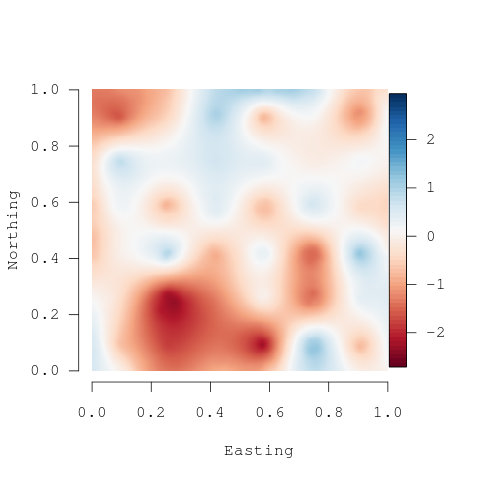
\includegraphics[width=3.5cm]{../figures/w-pp64.png}\label{uni-pp64-gs}}\\
				\end{center}
				\caption{Comparing full GP vs low-rank GP with 2500 locations} %Figure (\ref{uni-pp64-gs}) exhibits oversmoothing by a low-rank process (Predictive Process with 64 knots)} %\label{fig:uni-w}
		\end{figure}
			\vskip -8mm 	\begin{itemize}
					\item Low rank models like the Predictive Process (PP) often tends to oversmooth
					\item Increasing the number of knots can fix this but will lead to heavy computation
				\end{itemize}
			\end{alertblock}
	}
\end{frame}

\begin{frame}{Sparse matrices}
	\begin{itemize}
		\item \red{Idea:} Use a \blue{sparse} matrix instead of a low rank matrix to approximate the dense full GP covariance matrix
		\myitem \red{Goals:} 
		\begin{itemize} 
			\item Scalability: Both in terms of \blue{storage} and computing \blue{inverse} and \blue{determinants}
			\item Closely approximate full GP inference
			\item Proper Gaussian process model like the Predictive Process
	\end{itemize}
\end{itemize}
\end{frame}

\begin{frame}{Cholesky factors}
	\begin{itemize}\setlength{\itemsep}{0.4cm}
		\item Write a joint density $p(w) = p(w_1,w_2,\ldots,w_n)$ as:
		\[
		p(w_1)p(w_2\given w_1)\only<1-2>{p(w_3\given w_1, w_2)} \only<3>{\alert{p(w_3\given w_1, w_2)}} \cdots p(w_n\given w_1,w_2,\ldots,w_{n-1})
		\]
		 \item For Gaussian distribution $w \sim N(0,C)$ this $\Rightarrow$
		\only<1>{\begin{align*}
		w_1 &= 0 + \eta_1; \\
		w_2 &= a_{21}w_1 + \eta_2; \\
		\cdots & \qquad \cdots \qquad \cdots\\
		w_n & = a_{n1}w_1 + a_{n2}w_2 +  \cdots + a_{n,n-1}w_{n-1} + \eta_n; \\
		%\Longrightarrow w &= Aw + \eta;\quad \eta \sim N(0, D)
		\end{align*}}
		\only<2->{\begin{align*}
		\begin{bmatrix} w_1 \\ w_2 \\ w_3 \\ \vdots \\ w_n \end{bmatrix} &= \begin{bmatrix} 0 & 0 & 0 & \ldots & 0 & 0 \\ a_{21} & 0 & 0 & \ldots & 0 & 0\\ 
	    \only<2>{a_{31}}\only<3>{\alert{a_{31}}} & \only<2>{a_{32}}\only<3>{\alert{a_{32}}} & 0 & \ldots & 0 & 0 \\ \vdots & \vdots & \vdots & \vdots & \vdots & \vdots \\ a_{n1} & a_{n2} & a_{n3} & \ldots & a_{n,n-1} & 0\end{bmatrix}\begin{bmatrix} w_1 \\ w_2 \\ w_3 \\ \vdots \\ w_n \end{bmatrix} + \begin{bmatrix} \eta_1 \\ \eta_2 \\ \only<2>{\eta_3}\only<3>{\alert{\eta_3}} \\ \vdots \\ \eta_n \end{bmatrix} \\
		\Longrightarrow w &= Aw + \eta;\quad \eta \sim N(0, D),\; \mbox{where } D=diag(d_1,d_2,\ldots,d_n).
		\end{align*}}
		\only<3> {\item \red{Cholesky factorization:} $C^{-1} = (I-A)' D^{-1} (I-A)$}
	\end{itemize}
\end{frame}

\begin{frame}{Cholesky factors}
	\begin{itemize}
		\item $w_{<i}=(w_1,w_2,\ldots,w_{i-1})'$
		\item $c_i = Cov(w_i, w_{<i})$, $C_i = Var(w_{<i})$
		\item $i^{th}$ row of $A$ and $d_i=Var(\eta_i)$ are obtained from $p(w_i \given w_{<i})$ as follows:
			\begin{itemize}[<+-> ]
				\item Solve for $a_{ij}$'s from $\sum_{j=1}^{i-1} a_{ij} w_j = E(w_i \given w_{<i}) = c_i'C_i^{-1}w_{<i}$
				\item $d_i = Var(w_i \given w_{<i}) = \sigs - c_i'C_i^{-1}c_i$
			\end{itemize}
		\pause \item For large $i$, inverting $C_i$ becomes \red{slow}
		\item The Cholesky factor approach for the full GP covariance matrix $C$ \red{does not} offer any computational benefits
	\end{itemize}
\end{frame}

\begin{frame}{Cholesky Factors and Directed Acyclic Graphs (DAGs)}
		\begin{center}
		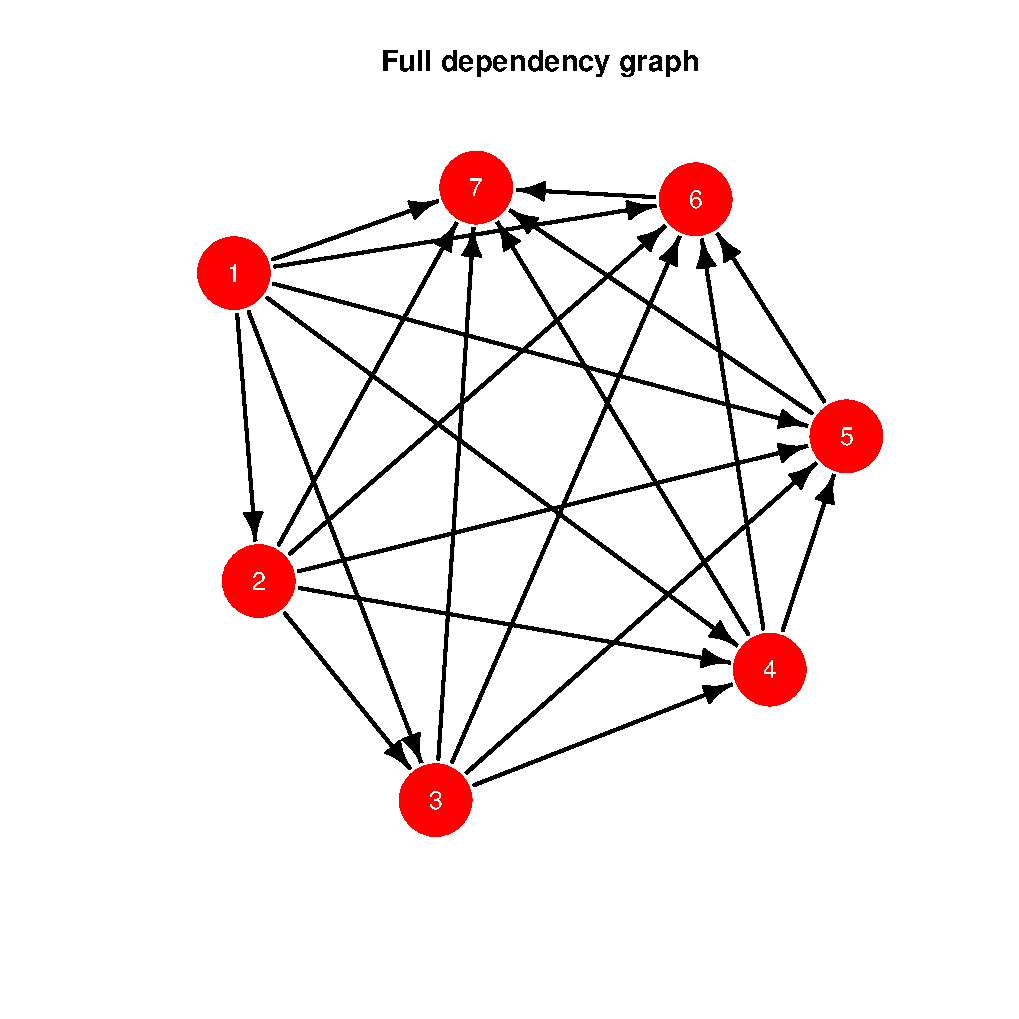
\includegraphics[scale=0.35, trim={0 1cm 1cm 2cm}, clip]{../figures/nnfull.pdf}
	\end{center}
	\begin{itemize}
		\item Number of non-zero entries (\alert{sparsity}) of $A$ equals number of arrows in the graph
		\item In particular: Sparsity of the $i^{th}$ row of $A$ is same as the number of arrows towards $i$ in the DAG
	\end{itemize}
\end{frame}

\begin{frame}{Introducing sparsity via graphical models}
	
	\only<1> 	{\begin{center}
	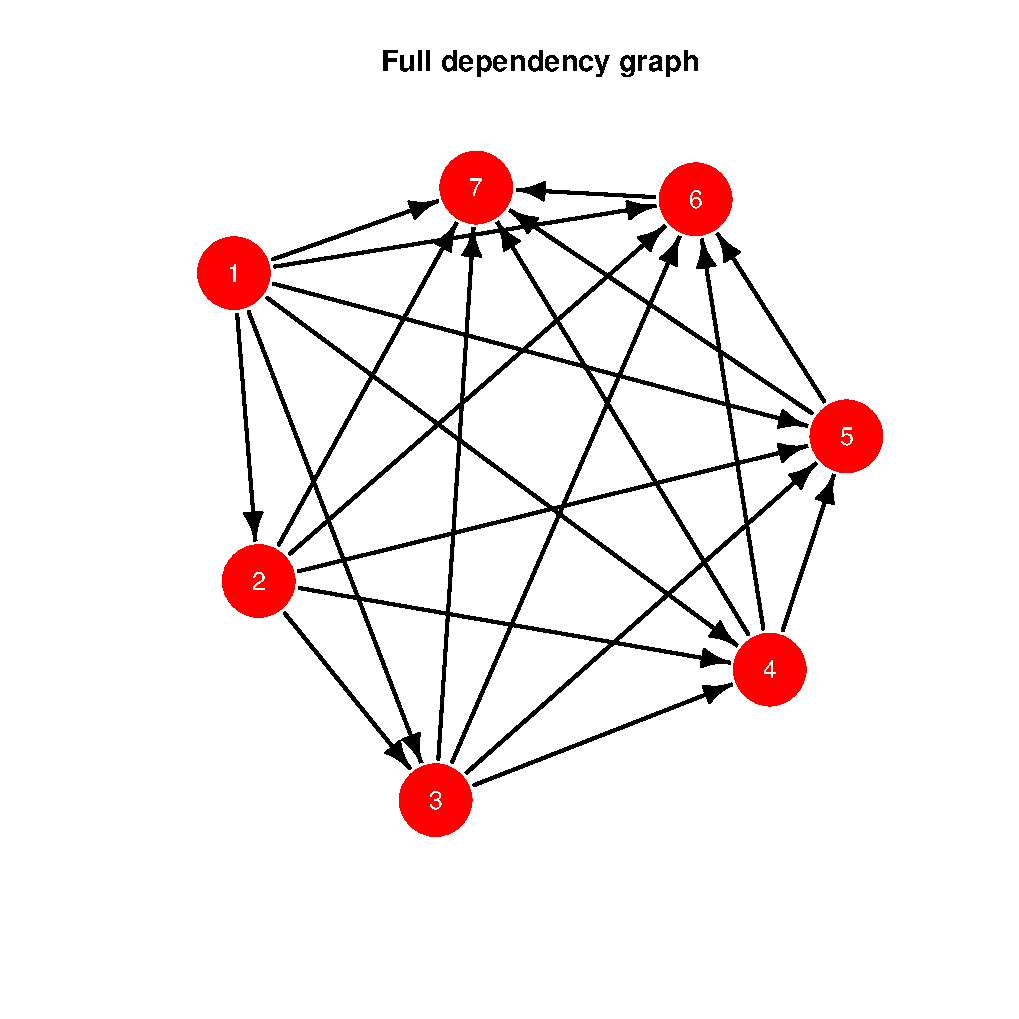
\includegraphics[scale=0.35, trim={0 1cm 1cm 2cm}, clip]{../figures/nnfull.pdf}
\end{center}
	{\small
	\begin{align*}
	& p(y_1)p(y_2\given y_1)p(y_3\given y_1,y_2)p(y_4\given y_1,y_2,y_3)\\ 
	&\qquad \times p(y_5\given y_1,y_2,y_3,y_4)p(y_6\given y_1,y_2,\ldots,y_5)  p(y_7\given y_1,y_2,\ldots,y_6)\;. 
	\end{align*}
}}
	\only<2> 	{\begin{center}
		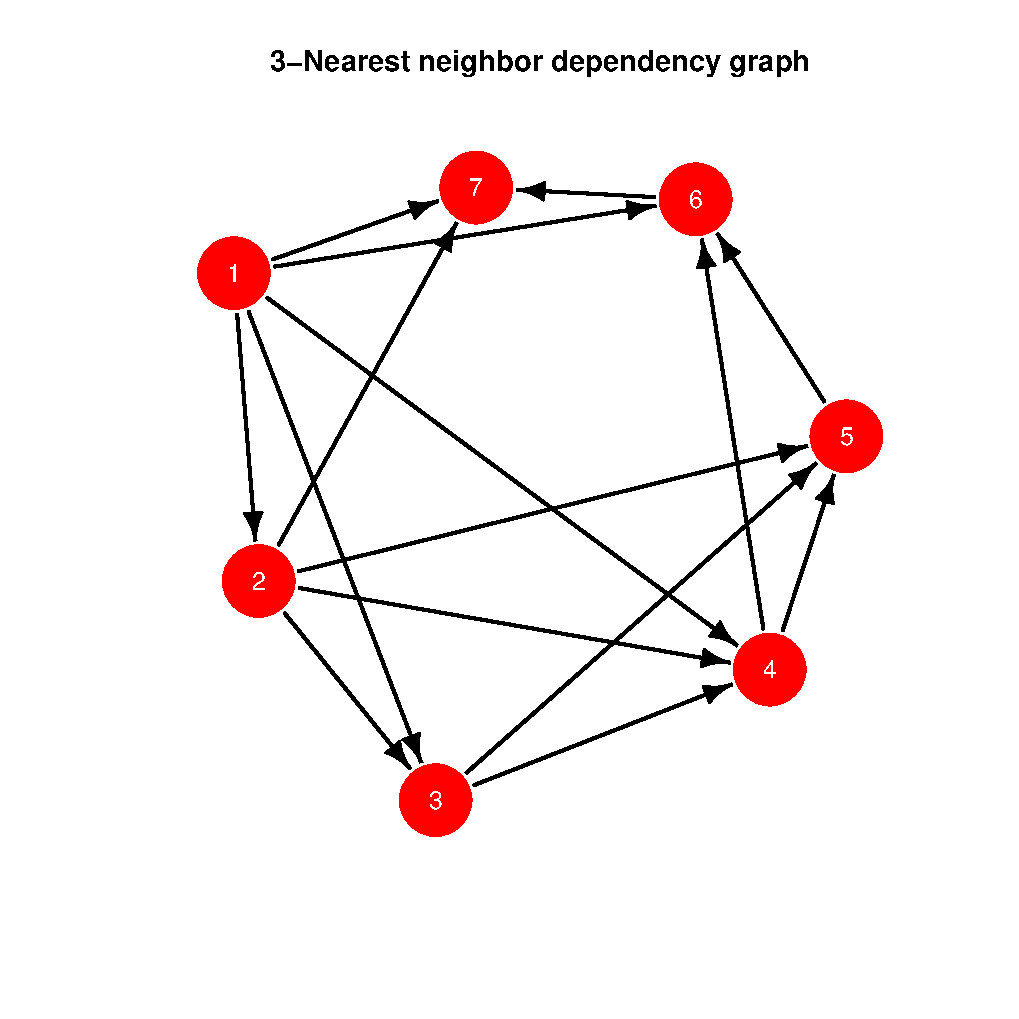
\includegraphics[scale=0.35, trim={0 1cm 1cm 2cm}, clip]{../figures/nn3.pdf}
\end{center}
	\small
		\begin{align*}
		& p(y_1)p(y_2\given y_1)p(y_3\given y_1,y_2)p(y_4\given y_1,y_2,y_3) \\ 
		& \qquad p(y_5\given \cancel{y_1}, y_2,y_3,y_4) p(y_6\given y_1, \cancel{y_2},\cancel{y_3}, y_4,y_5) p(y_7\given y_1,y_2,\cancel{y_3},\cancel{y_4},\cancel{y_5}, y_6) 
		\end{align*}
	}
\end{frame}

\begin{frame}{Introducing sparsity via graphical models}
	\begin{center}
		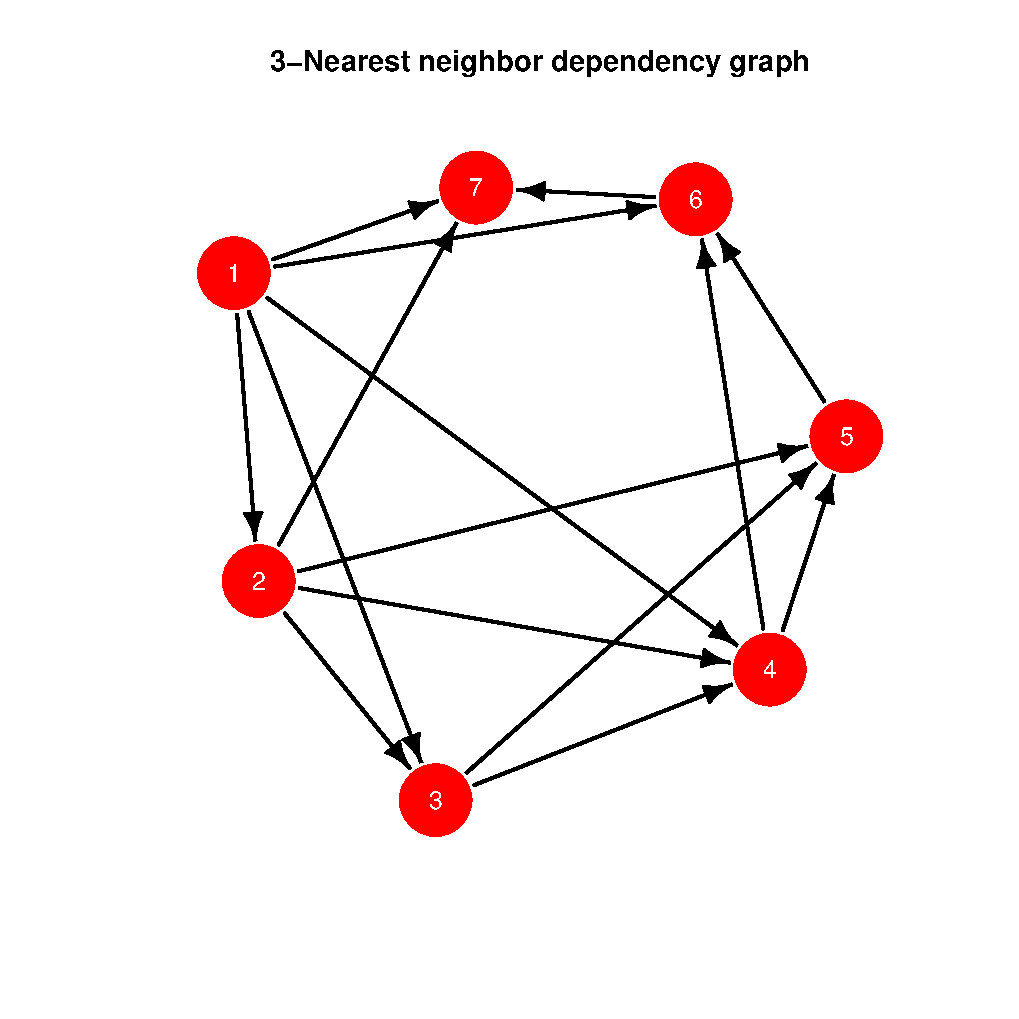
\includegraphics[scale=0.35, trim={0 1cm 1cm 2cm}, clip]{../figures/nn3.pdf}
	\end{center}
\vskip -10mm \begin{itemize}
	\only<1>{
	\item Create a \alert{sparse} DAG by keeping \red{at most $m$} arrows pointing to each node
	\item Set $a_{ij}=0$ for all $i,j$ which has no arrow between them 
	\item Fixing $a_{ij}=0$ introduces \blue{conditional independence} and $w_j$ drops out from the conditional set in $p(w_i\given \{w_k: l < i\})$
	}
	\only<2>{
		\item $N(i)$ denote \alert{\em{neighbor set}} of $i$, i.e., the set of nodes from which there are arrows to $i$
		 \item $a_{ij}=0$ for $j \notin N(i)$ and nonzero $a_{ij}$'s obtained by solving: 
		\[
		\mbox{E}[w_i\given w_{N(i)}] = \sum_{j \in N(i)}a_{ij}w_j
		\]
		\item The above linear system is only \red{$m\times m$}
	}
\end{itemize}
\end{frame}

\begin{frame}{Choosing neighbor sets}
	Matern Covariance Function: 
	\begin{equation*}\label{matern}
	C(s_i, s_j) = \frac{1}{2^{\nu - 1}\Gamma(\nu)}(||s_i-s_j||\phi)^{\nu}\calK_{\nu}(||s_i-s_j||\phi);\; \phi > 0, \nu >0,
	\end{equation*}
	\begin{figure}
		\centering
		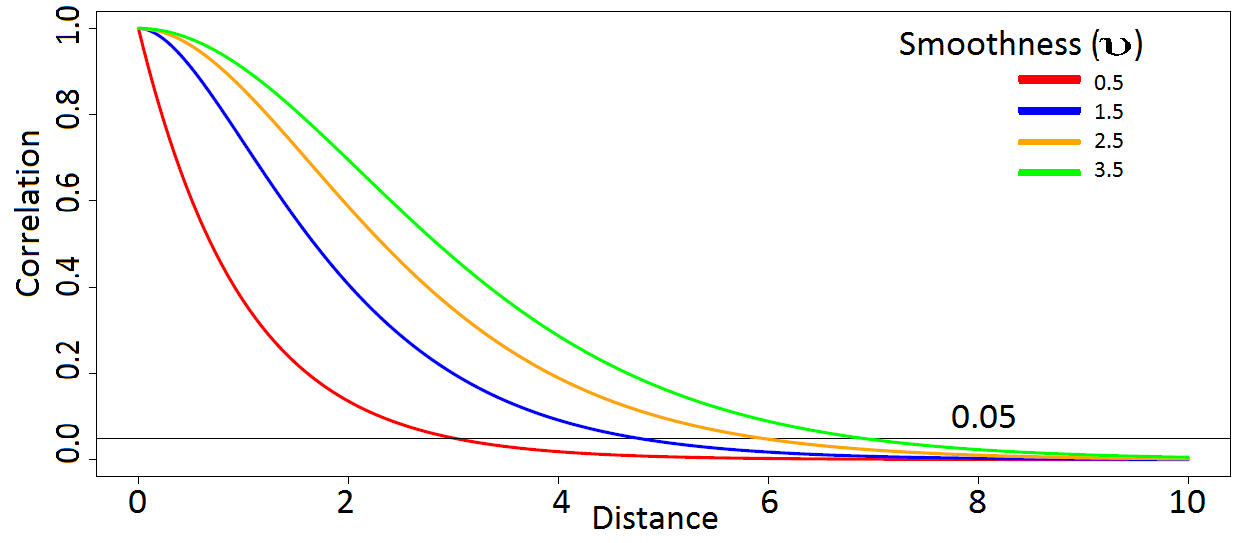
\includegraphics[width=10cm]{../figures/matern.png}
		%\vskip -3mm \caption{Matern covariance functions decreasing with distance}
	\end{figure}
\end{frame}

\begin{frame}{Choosing neighbor sets}
	\begin{itemize}
		\item Spatial covariance functions decay with distance
		\myitem Vecchia (1988): $N(s_i) =$ \red{$m-$nearest neighbors} of $s_i$ in $s_1, s_2, \ldots, s_{i-1}$
		\begin{itemize}
			\myitem Nearest points have highest correlations
			\myitem Theory: \blue{"Screening effect"} -- Stein, 2002
		\end{itemize}
		\item We use Vecchia's choice of $m$-nearest neighbor
		\myitem Other choices proposed in Stein et al. (2004); Gramacy and Apley (2015); Guinness (2016) can also be used
	\end{itemize}
\end{frame}

\begin{frame}{Nearest neighbors}
	\only<1>{\centering 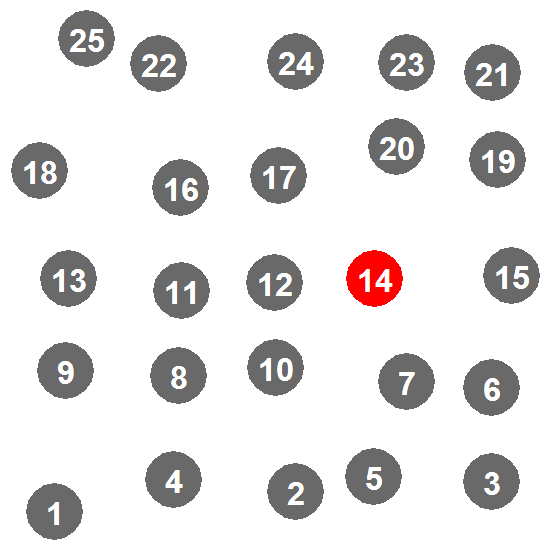
\includegraphics[scale=0.25,trim={0cm 0cm 0cm 0cm},clip]{../figures/nnnew.png}}
	\only<2>{\centering 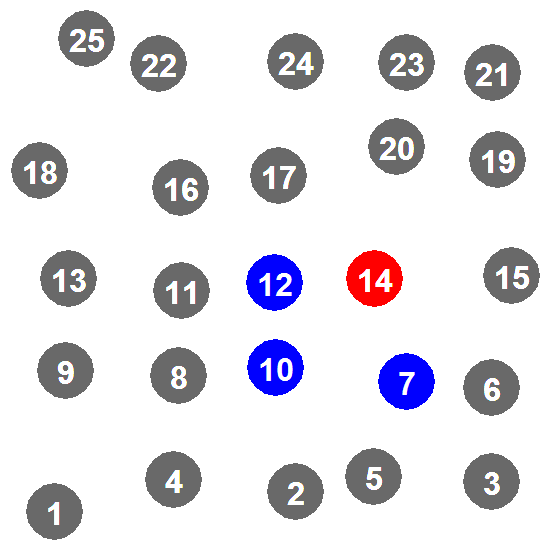
\includegraphics[scale=0.25,trim={0cm 0cm 0cm 0cm},clip]{../figures/nnnew14.png}}
	%\only<3>{\centering 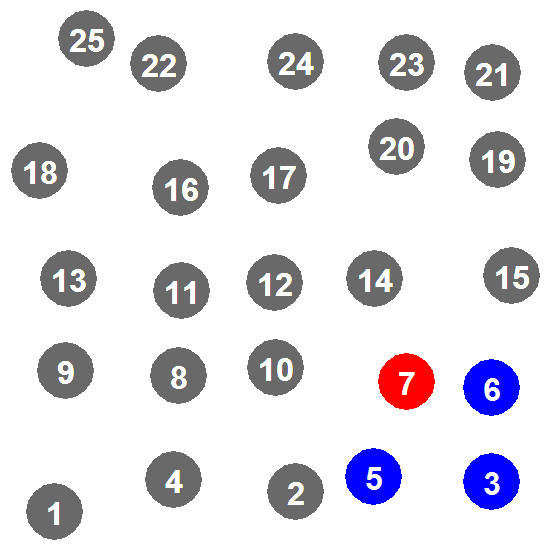
\includegraphics[scale=0.25,trim={0cm 0cm 0cm 0cm},clip]{../figures/nnnew7.png}}
	\only<3>{\centering 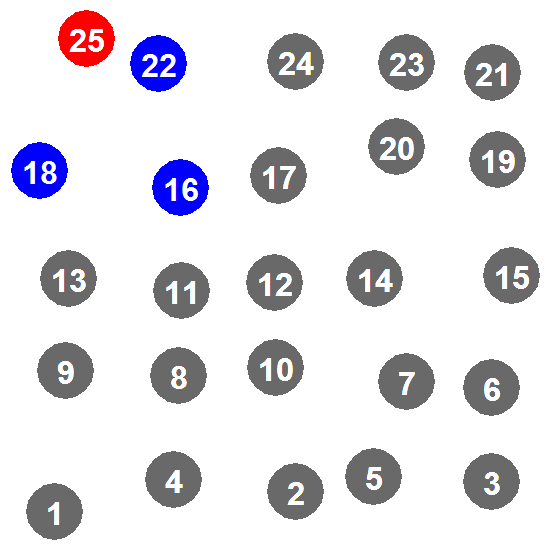
\includegraphics[scale=0.25,trim={0cm 0cm 0cm 0cm},clip]{../figures/nnnew25.png}}
\end{frame}

\begin{frame}{Sparse precision matrices}
	%\textcolor{red}{Result:}
\begin{itemize}
\item The neighbor sets and the covariance function $C(\cdot,\cdot)$ define a sparse Cholesky factor $A$
\item \alert{$N(w \given 0, C) \approx N(w \given 0, \tilde C)\; ; \tilde C^{-1} = (I-A)^{\top} D^{-1} (I-A)$
			}
\end{itemize}		
	\only<1>{
		\vskip -6mm \begin{figure}
			\centering
			\hskip -4mm \subfloat[A]{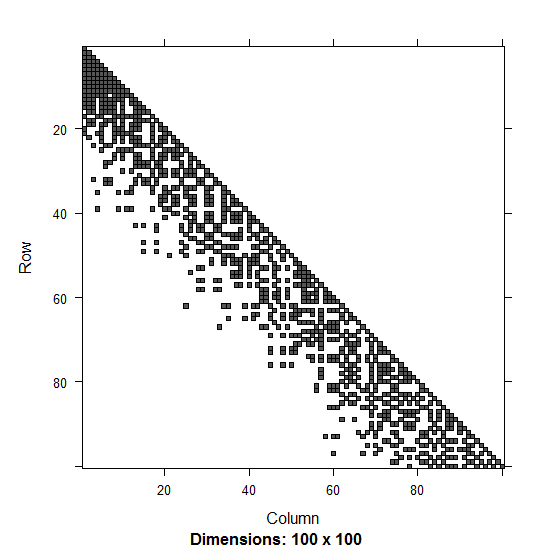
\includegraphics[width=3.5cm,trim={2.4cm 2.4cm 0cm 0cm},clip]{../figures/v100.png}}
			\subfloat[D]{ 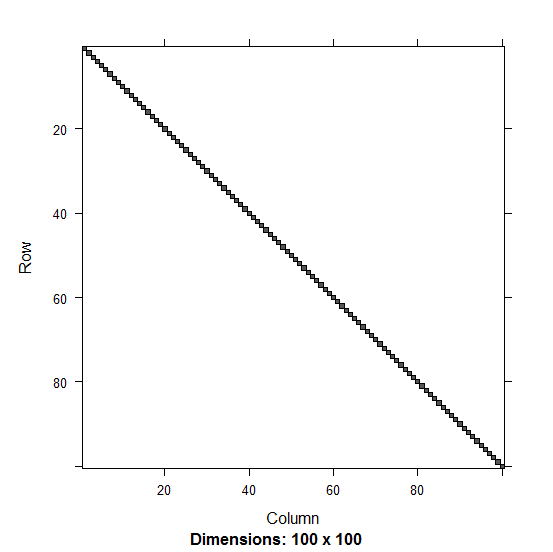
\includegraphics[width=3.5cm,trim={2.4cm 2.4cm 0cm 0cm},clip]{../figures/f.png}}
			\subfloat[$\tilde C^{-1}$]{  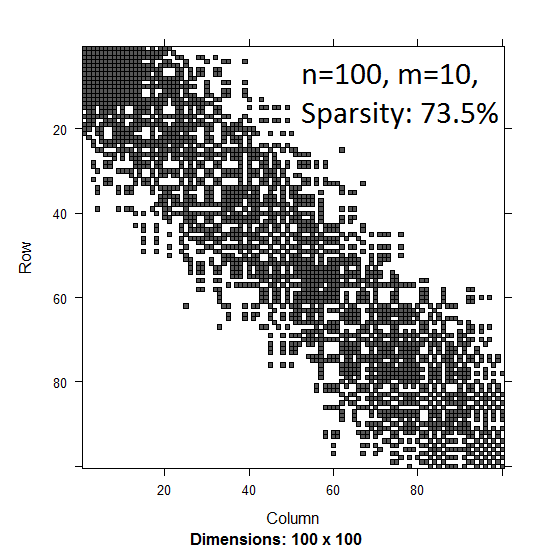
\includegraphics[width=3.5cm,trim={2cm 2cm 0cm 0cm},clip]{../figures/q100.png}}
		\end{figure}
	}

\only<2>{
	\vskip -4mm \begin{figure}
		\centering
		\hskip -4mm \subfloat[A]{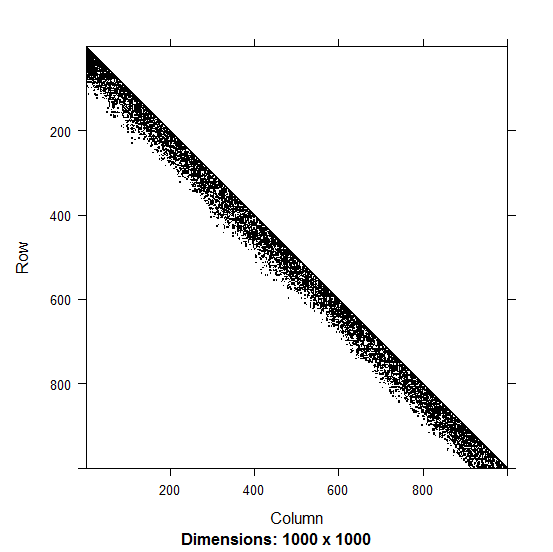
\includegraphics[width=3cm,trim={2.4cm 2.4cm 0cm 0cm},clip]{../figures/v1000.png}}
		\subfloat[D]{ 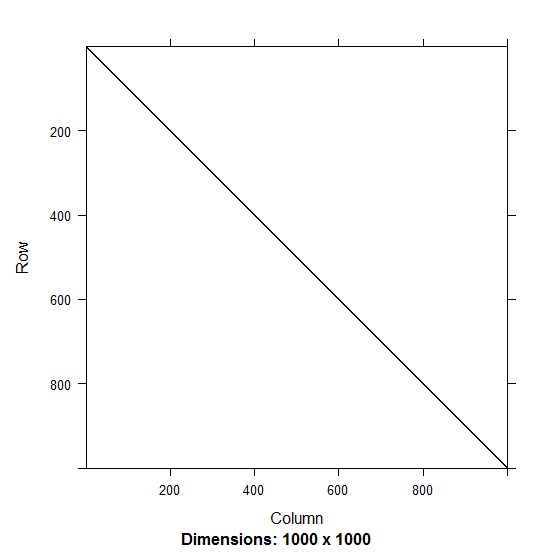
\includegraphics[width=3cm,trim={2.4cm 2.4cm 0cm 0cm},clip]{../figures/f1000.png}}
		\subfloat[$\tilde C^{-1}$]{  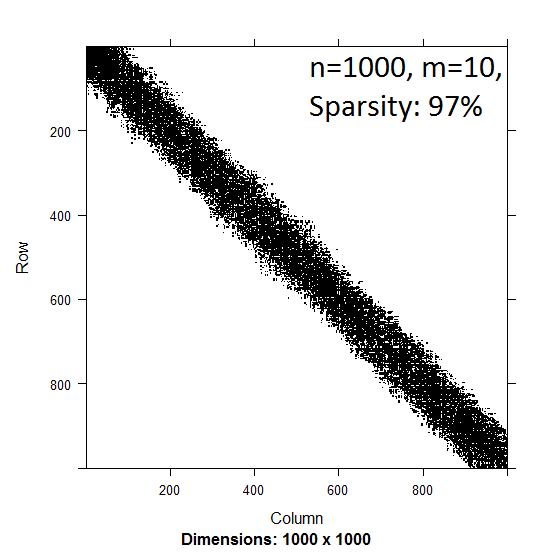
\includegraphics[width=3cm,trim={2cm 2cm 0cm 0cm},clip]{../figures/q1000.png}}
	\end{figure}
}
\vspace{-0.25cm}

\begin{itemize}%\setlength{\itemsep}{0.2cm}
		%\item Cholesky: $\tkt^{-1}=V F V^{\top}$
		%\item $V$ and $F$ are obtained from $w(s,t_i) \given w_{N(s,t_i)}$'s
		\item $\det(\tilde C) = \prod_{i=1}^n D_{i}$,  %$|N(s,t_i)| \leq m \ll n  \Rightarrow$ 
		\item $\tilde C^{-1}$ is sparse with \textcolor{blue}{$O(nm^2)$} entries
                \item Explore some $A$ and $\tilde C^{-1}$ sparsity patterns \textcolor{blue}{\url{https://github.com/finleya/NNGP_LDL}}
\end{itemize}

\end{frame}

\begin{frame}{Extension to a Process} %(Datta et al., \emph{JASA}, 2015)}
	\begin{itemize}\setlength{\itemsep}{1cm}
		\item We have defined $w \sim N(0, \tilde C)$ over the set of data locations $S=\{s_1, s_2, \ldots, s_n\}$
		\item For $s \notin S$, define $N(s)$ as set of $m$-nearest neighbors of $s$ in $S$
		\item Define $w(s) = \sum_{i:s_i \in N(s)} a_i(s)w(s_i) + \eta(s)$ where $\eta(s) \ind N(0,d(s))$ 
		\begin{itemize}
			\item $a_i(s)$ and $d(s)$ are once again obtained by solving $m \times m$ system
		\end{itemize}
		\item Well-defined GP over entire domain
		\begin{itemize}
			\item \textcolor{blue}{Nearest Neighbor GP (NNGP)} -- Datta et al., JASA, (2016)
		\end{itemize}
		%\item Nonzero $a_i(s)$'s: solve $m\times m$ system $K_{N(s),N(s)}a_{N(s)} = K_{N(s),s} $.
	\end{itemize}
\end{frame}

\begin{frame}{Hierarchical spatial regression with NNGP}
	\metroset{block=fill}
	\begin{alertblock}{Spatial linear model}
	\[y(\bs)=x(\bs)'\beta + w(\bs) + \eps(\bs)\]
\end{alertblock}
\begin{itemize}
\item $w(s)$ modeled as $NNGP$ derived from a $GP(0, C(\cdot, \cdot, \given \sigs, \phi))$
\item $\eps(s) \iid N(0,\taus)$ contributes to the nugget
\item Priors for the parameters $\beta$, $\sigs$, $\taus$ and $\phi$
\item \red{Only} difference from a full GP model is the NNGP prior $w(s)$
\end{itemize}
\end{frame}

\begin{frame}{Hierarchical spatial regression with NNGP}
	\metroset{block=fill}
\vskip 2mm \begin{alertblock}{Full Bayesian Model}
		\begin{align*}
		N(y &\given X\beta +w, \tau^2I) \times N(w\given 0,\tilde C(\sigs, \phi)) \times N(\beta \given \mu_\beta,V_\beta)\\
		& \times IG(\tau^2 \given a_\tau,b_\tau) \times IG(\sigs \given a_\sigma,b_\sigma) \times Unif(\phi \given a_\phi, b_\phi)
		\end{align*} 
\end{alertblock}
Gibbs sampler:
	\begin{itemize}
		\item Conjugate full conditionals for $\beta$, $\tau^2$, $\sigs$ and $w(s_i)$'s 
		\item Metropolis step for updating $\phi$
		\item \blue{Posterior predictive distribution} at any location using composition sampling:
		\begin{small}
		\begin{align*}
		\hskip -1cm  \int N(y(s) \given &x(s)'\beta + w(s), \tau^2I) \times N(w(s) \given a(s)'w_{R}, d(s)) \times \\
		&p(w, \beta, \taus, \sigs, \phi \given y) \, d(w,\beta, \taus, \sigs, \phi)
		\end{align*} 
		\end{small}
	\end{itemize}
\end{frame}

\begin{frame}{Choosing $m$}
	\begin{figure}[t!]
		\begin{center}
			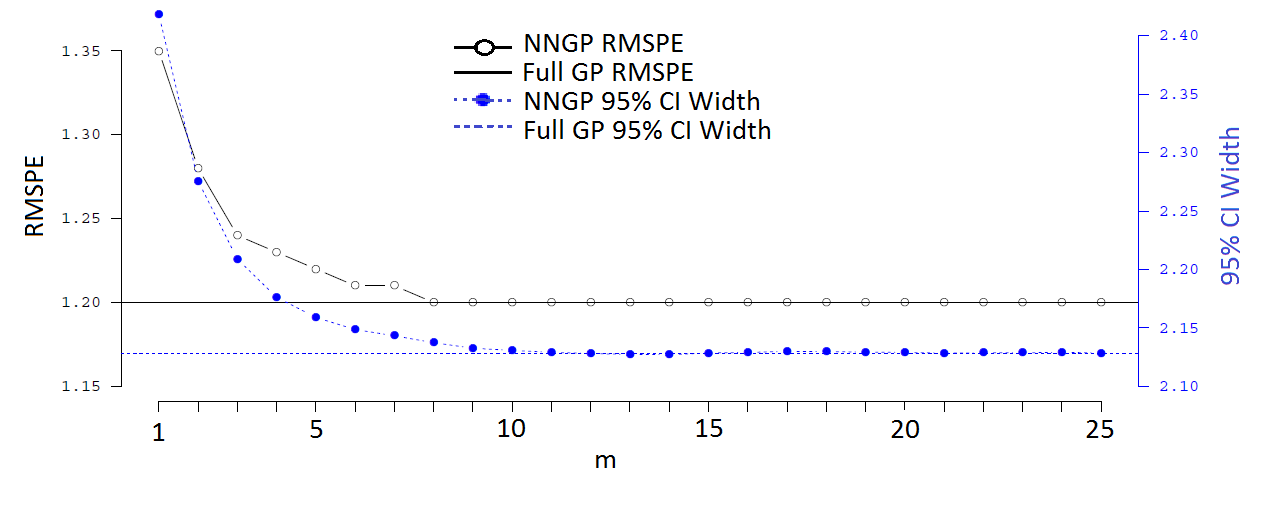
\includegraphics[width=10cm]{../figures/nn-pred.png}\label{uni-nn-pred}
		\end{center}
	\end{figure}
	
	\begin{itemize}
		\item Run NNGP in parallel for few values of $m$
		\myitem Choose $m$ based on model evaluation metrics
		\myitem Our results suggested that typically $m \approx 20$ yielded excellent approximations to the full GP
	\end{itemize}
\end{frame}

\begin{frame}{Storage and computation}
	\begin{itemize}\setlength{\itemsep}{0.4cm}
		\item Storage:
		\begin{itemize}
			\item \red{Never} needs to store $n \times n$ distance matrix 
			\item Stores smaller $m \times m$ matrices %(can be overwritten to save space)
			\item Total storage requirements \red{$O(nm^2)$}
		\end{itemize}
		\item Computation:
		\begin{itemize}
			\item Only involves inverting small $m \times m $ matrices
			\item Total flop count per iteration of Gibbs sampler is \red{$O(nm^3)$} 
		\end{itemize}
	\item Since \red{$m \ll n$}, NNGP offers great \blue{scalability} for large datasets
	\end{itemize}
\end{frame}


\begin{frame}{Simulation experiments}
	\begin{itemize}
		\item $2500$ locations on a unit square \vskip 2mm
		\myitem $y(s) = \beta_0 + \beta_1 x(s) + w(s) + \eps(s)$ \vskip 2mm
		\myitem Single covariate $x(s)$ generated as iid $N(0,1)$ \vskip 2mm
		\myitem Spatial effects generated from $GP(0, \sigma^2 R(\cdot, \cdot \given \phi))$ \vskip 2mm
		\myitem $R(\cdot,\cdot \given \phi)$ is exponential correlation function with decay $\phi$ \vskip 2mm
		\myitem Candidate models: Full GP, Gaussian Predictive Process (GPP) with 64 knots and NNGP \vskip 2mm
	\end{itemize}
\end{frame}

\begin{frame}{Fitted Surfaces}
	\begin{figure}[t]
		\vskip -4mm \begin{center}
			\subfloat[True $w$]{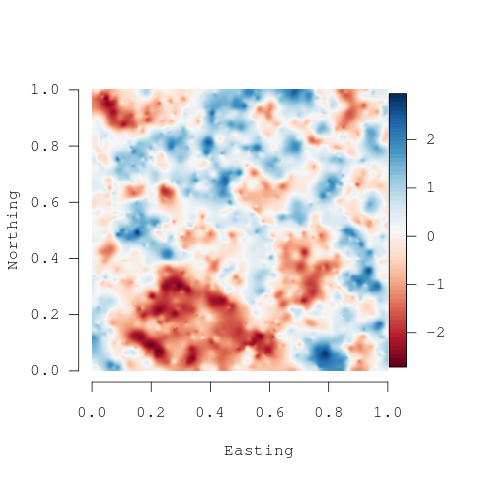
\includegraphics[width=3cm]{../figures/w-obs.png}\label{uni-w-obs}}
			\subfloat[Full GP]{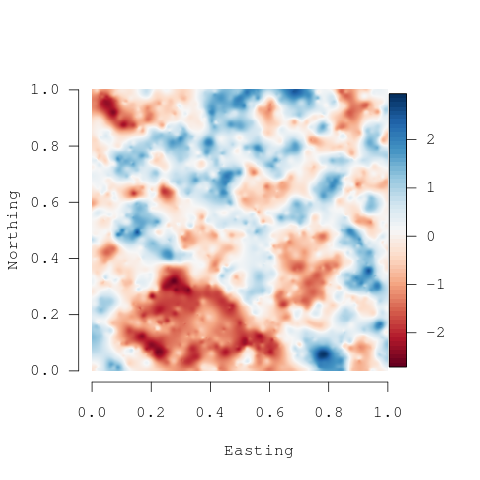
\includegraphics[width=3cm]{../figures/w-gs.png}\label{uni-w-gs}}
			\subfloat[GPP 64 knots]{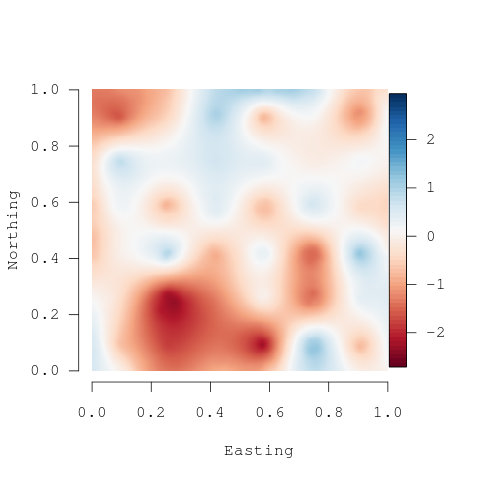
\includegraphics[width=3cm]{../figures/w-pp64.png}\label{uni-pp64-gs}}\\ 
			\subfloat[NNGP, $m=10$]{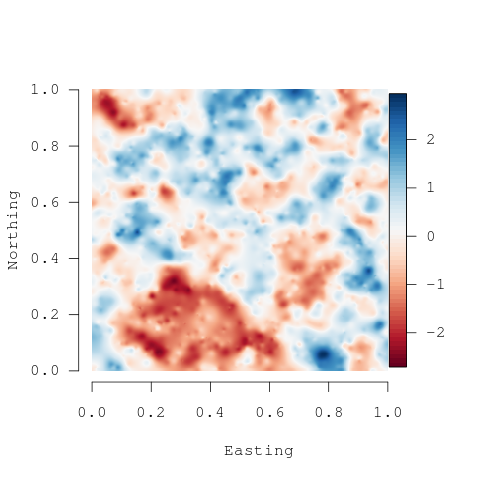
\includegraphics[width=3cm]{../figures/w-k10.png}\label{uni-k10-gs}} \hspace{4mm}
			\subfloat[NNGP, $m=20$]{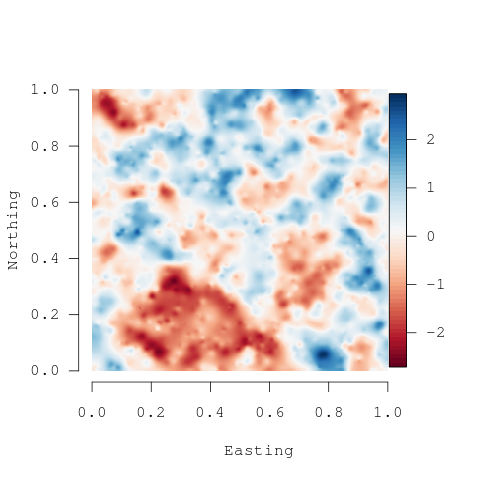
\includegraphics[width=3cm]{../figures/w-k20.png}\label{uni-k20-gs}} \hspace{4mm}
		\end{center}
		\caption{Univariate synthetic data analysis} \label{fig:uni-w}
	\end{figure}
\end{frame}

\begin{frame}{Parameter estimates}
	\begin{table}[]
		\centering
		%\caption{Univariate synthetic data analysis}
		{\tiny
			\begin{tabular}{cccccc}
				\hline
				&       &\multicolumn{2}{c}{NNGP} &Predictive Process &Full\\
				& True            &$m=10$ & $m=20$           &64 knots          & Gaussian Process \\ 
				\hline
				$\beta_{0}$ &1&1.00 (0.62, 1.31)&1.03 (0.65, 1.34)&1.30 (0.54, 2.03)&1.03 (0.69, 1.34)\\ 
				$\beta_{1}$  &5&5.01 (4.99, 5.03)&5.01 (4.99, 5.03)&5.03 (4.99, 5.06)&5.01 (4.99, 5.03)\\ 
				$\sigma^2$  &1&0.96 (0.78, 1.23)&0.94 (0.77, 1.20)&1.29 (0.96, 2.00)&0.94 (0.76, 1.23)\\ 
				$\tau^2$  &0.1&0.10 (0.08, 0.13)&0.10 (0.08, 0.13)&0.08 (0.04, 0.13)&0.10 (0.08, 0.12)\\ 
				$\phi$  &12&12.93 (9.70, 16.77)&13.36 (9.99, 17.15)&\textcolor{red}{5.61 (3.48, 8.09)}&13.52 (9.92, 17.50)\\ 
				\hline
			\end{tabular}
		}
	\end{table}
	%%\end{table}
\end{frame}

\begin{frame}{Model evaluation}
	\begin{table}[]
		\centering
		%\caption{Univariate synthetic data analysis}
		{\scriptsize
			\begin{tabular}{ccccc}
				\hline
				&\multicolumn{2}{c}{NNGP} &Predictive Process &Full\\
				&$m=10$ & $m=20$           &64 knots          & Gaussian Process \\ 
				\hline
				%  p$_D$  &--&1243.32&1249.57&1258.27&1260.68\\ 
				%  DIC &--&2390.65&2377.51&\textcolor{red}{13677.97}&2364.80\\
				% G (Goodness of fit) &--&77.84&76.40&1075.63&74.80\\
				% P (Penalization) &--&340.40&337.88&200.39&333.27\\
				DIC score &2390&2377&\textcolor{red}{13678}&2364\\
				RMSPE &1.2&1.2&\textcolor{red}{1.68}&1.2\\  \hline
				%Wall Time  &--&20.79&66.74&14.44&46.85&2.24&29.91\\
				Run time (Minutes) &\textcolor{blue}{14.40}&46.47&43.36&\textcolor{red}{560.31}\\
				%System time &--&0.47&1.32&0.02&0.31&1.32&17.28\\
				\hline
			\end{tabular}
		}
	\end{table}
	%%\end{table}
	
	\begin{itemize}
		%\item Parameter estimates for all models are similar
		\item NNGP performs at par with Full GP
		\item GPP oversmooths and performs much worse both in terms of parameter estimation and model comparison
		\item NNGP yields huge computational gains
	\end{itemize}
\end{frame}

% \begin{frame}{Multivariate spatial data}
% 
% \begin{itemize}
% \item Point-referenced spatial data often come as \red{ multivariate measurements} at each location.%\pause
% 
% \item \blue {Examples:}
% \begin{itemize}
% \item \red{Environmental monitoring}: stations yield measurements on \blue{ozone}, \blue{NO}, \blue{CO}, and \blue{$\text{PM}_{2.5}$}.%\pause
% 
% %\item \red{Community ecology}: assemblages of plant species due to \blue{water availibility}, \blue{temperature}, and \blue{light} requirements.%\pause
% 
% \item \red{Forestry}: measurements of stand characteristics \blue{age}, \blue{total biomass}, and \blue{average tree diameter}.%\pause
% 
% \item \red{Atmospheric modeling}: at a given site we observe \blue{surface temperature}, \blue{precipitation} and \blue{wind speed}%\pause
% 
% \end{itemize}
% 
% \item We anticipate dependence between measurements %\pause
% \begin{itemize}
% \item \red{at a particular location}%\pause
% 
% \item \blue{across locations}
% \end{itemize}
% \end{itemize}
% \end{frame}
% 
% \begin{frame}{Multvariate spatial linear model}
% \begin{itemize}
% \item Spatial linear model for $q$-variate spatial data:
% $y_i = x_i'(s)\beta_i + w_i(s) + \eps_i(s)$ for $i=1,2,\ldots,q$
% \myitem $\eps(s) = (\eps_1(s),\eps_2(s),\ldots,\eps_q(s))' \sim N(0,E)$ where $E$ is the $q \times q$ noise matrix
% \myitem $w(s) = (w_1(s), w_2(s), \ldots, w_q(s))'$ is modeled as a $q$-variate  Gaussian process
% \end{itemize}
% \end{frame}

\begin{frame}{Spatially varying coefficients}
\begin{itemize}
\item Often the relationship between the (univariate) spatial response and covariates vary across the space
\item The regression coefficients can then be modeled as spatial processes
\item \alert{Spatially varying coefficient (SVC)} model: 
$y(s) = x(s)'\beta\red{(s)} + \eps(s)$
\item Even though the response can be univariate, 
$\beta(s)$ is modeled as a $p$-variate GP
\end{itemize}
\end{frame}

\begin{frame}{Multivariate GPs}
\begin{itemize}
\myitem $Cov(w(s_i),w(s_j)) = C(s_i,s_j \given \theta)$ -- a $q \times q$ \alert{cross-covariance} matrix
\myitem Choices for the function $C(\cdot, \cdot \given \theta)$
	\begin{itemize}
	\item Multivariate Mat\'ern
	\item Linear model of co-regionalization
	\end{itemize}
\myitem For data observed at $n$ locations, all choices lead to a dense \red{$nq \times nq$} matrix $C = Cov(w(s_1),w(s_2),\ldots,w(s_n))$
\myitem Not scalable when $nq$ is large
\end{itemize}
\end{frame}

\begin{frame}{Multivariate NNGPs}
\begin{itemize}
\item Cholesky factor approach similar to the univariate case
\begin{align*}
		\begin{bmatrix} w(s_1) \\ w(s_2) \\ w(s_3) \\ \vdots \\ w(s_n) \end{bmatrix} &= \begin{bmatrix} 0 & 0 & 0 & \ldots & 0 & 0 \\ A_{21} & 0 & 0 & \ldots & 0 & 0\\ 
A_{31} & A_{32} & 0 & \ldots & 0 & 0 \\ \vdots & \vdots & \vdots & \vdots & \vdots & \vdots \\ A_{n1} & A_{n2} & A_{n3} & \ldots & A_{n,n-1} & 0\end{bmatrix}\begin{bmatrix} w(s_1) \\ w(s_2) \\ w(s_3) \\ \vdots \\ w(s_n) \end{bmatrix} + \begin{bmatrix} \eta(s_1) \\ \eta(s_2) \\ \eta(s_3) \\ \vdots \\ \eta(s_n) \end{bmatrix} \\
		\Longrightarrow w &= Aw + \eta;\quad \eta \sim N(0, D),\;  D=diag(D_1,D_2,\ldots,D_n).
		\end{align*}
\item \red{Only differences:} $w(s_i)$ and $\eta(s_i)$'s are $q \times 1$ vectors and $A_{ij}$ and $D_i$'s are $q \times q$ matrix
\end{itemize}
\end{frame}

\begin{frame}{Multivariate NNGPs}
\begin{itemize}
\item Choose neighbor sets $N(i)$ for each location $s_i$
\myitem Set $A_{ij}=0$ if $j \notin N(i)$
\myitem Solve for non-zero $A_{ij}$'s from the \red{$mq \times mq$} linear system: $\sum_{j \in N(i)} A_{ij}w(s_j) = E(w(s_i) \given \{ w(s_j) \given j \in N(i) \})$
\myitem \alert{Multivariate NNGP:} $w \sim N(0, \tilde C)$ where $\tilde C^{-1} = (I-A)' D^{-1} (I-A)$
\myitem $\tilde C^{-1}$ is sparse with $O(nm^2)$ non-zero $q \times q$ blocks
\myitem $\det(\tilde C) = \prod_{i=1}^n \det(D_i)$
\myitem Storage and computation needs remains \red{linear} in $n$
\end{itemize}
\end{frame}

\begin{frame}{U.S. Forest biomass data}
\begin{figure}[]
\begin{center}
\vskip-4mm\subfloat[Observed biomass]{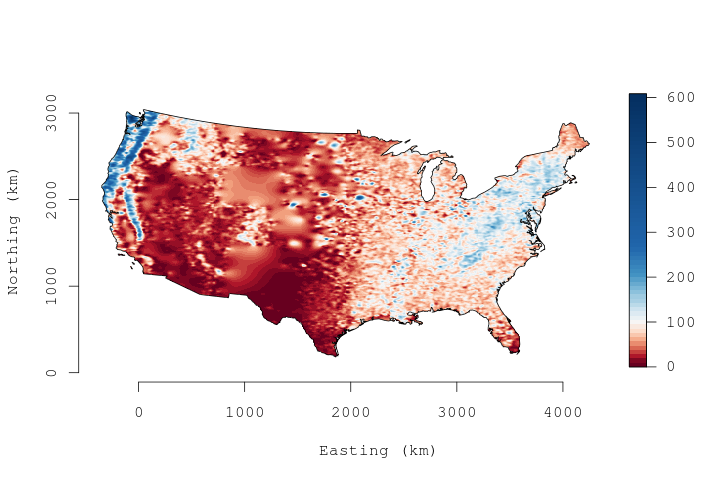
\includegraphics[width=5cm]{../figures/obs-biomass.png}\label{bio-obs}}
\subfloat[NDVI]{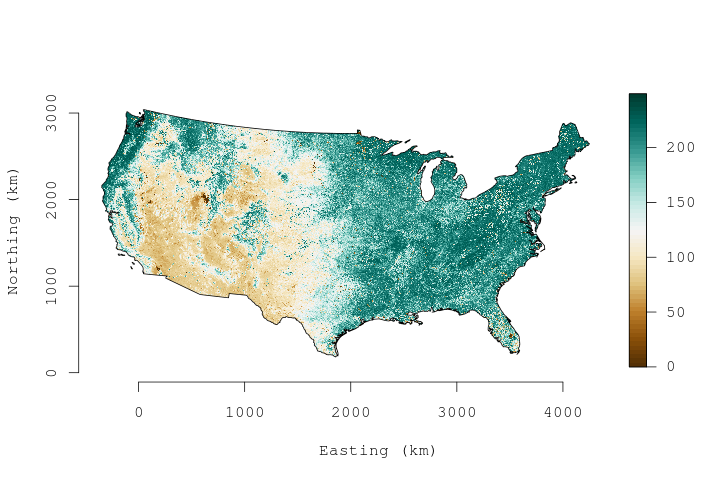
\includegraphics[width=5cm]{../figures/ndvi.png}\label{bio-ndvi}}
\end{center}
%\caption{Observed biomass (left) and NDVI (right)}\label{fig:bio}
\end{figure}
\begin{itemize}
\item Forest biomass data from measurements at 114,371 plots
%\item Normalized Difference Vegetation Index (NDVI) calculated in July 2006
\myitem NDVI (greenness) is used to predict forest biomass
\end{itemize}
\end{frame}

\begin{frame}{U.S. Forest biomass data}
  \begin{block}{Non Spatial Model}
$Biomass = \beta_0 + \beta_1 NDVI + error$, \hskip 2mm $\hat {\beta_0} = 1.043$, $\hat {\beta_1} = 0.0093$
\end{block}
\vskip-4mm
\begin{figure}[]
\begin{center}
\subfloat[Residuals]{{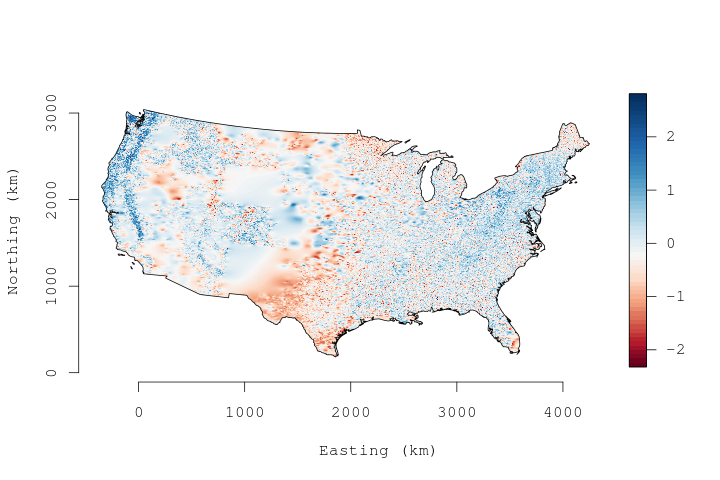
\includegraphics[width=5cm]{../figures/non-sp-resid.png}\label{nonspres}}}
\subfloat[Variogram of residuals]{{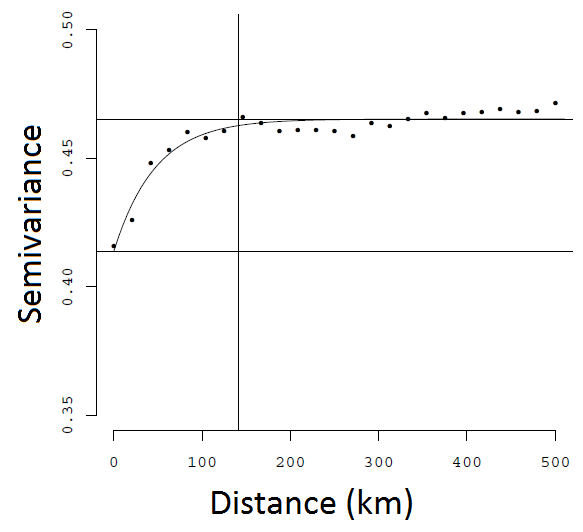
\includegraphics[height=3.5cm,width=5cm]{../figures/semiv.png}\label{vario}}}
\label{fig:biononsp}
%\vskip-4mm\caption{Heat map (left) and variogram (right) of residuals reflecting spatial correlation} 
\end{center}
\end{figure}
\begin{alertblock}{\centering Strong spatial pattern among residuals}
\end{alertblock}
\end{frame}

\begin{frame}{Forest biomass dataset}
\begin{itemize}
\item $n \approx 10^5$ (Forest Biomass) $\Rightarrow$ full GP requires storage \red{$\approx 40Gb$} and time \red{$\approx 140$ hrs} per iteration.
\myitem We use a spatially varying coefficients NNGP model
\end{itemize}

\begin{block}{Model}
\begin{itemize}
\item $Biomass(s)= \beta_0(s)+\beta_1(s)NDVI(s)+\epsilon(s)$
\myitem $w(s)=(\beta_0(s),\beta_1(s))^{\top} \sim $ \blue{Bivariate} $NNGP(0,\tilde C(\cdot,\cdot \given \theta))$, $m=5$
\myitem Time \red{$\approx 6$ seconds} per iteration
\myitem Full inferential output: $41$ hours ($25000$ MCMC iterations)
\end{itemize}
\end{block}
\end{frame}

\begin{frame}{Forest biomass data}

\begin{figure}[]
\begin{center}
\vskip -5mm
\subfloat[Observed biomass]{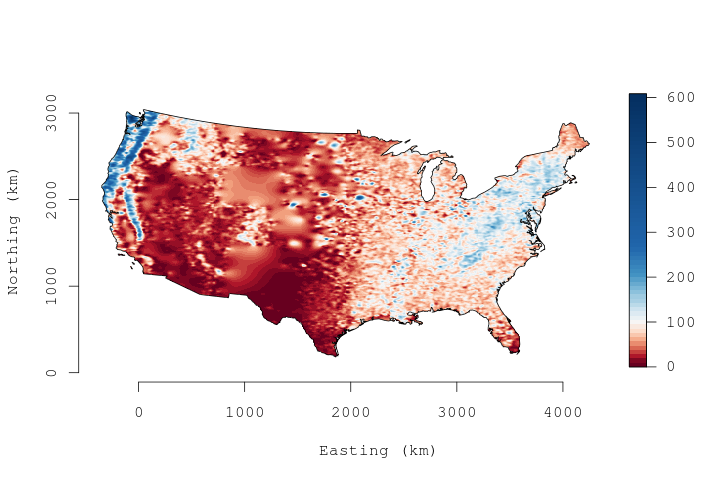
\includegraphics[width=5cm]{../figures/obs-biomass.png}\label{bio-obs}}
\subfloat[Fitted biomass]{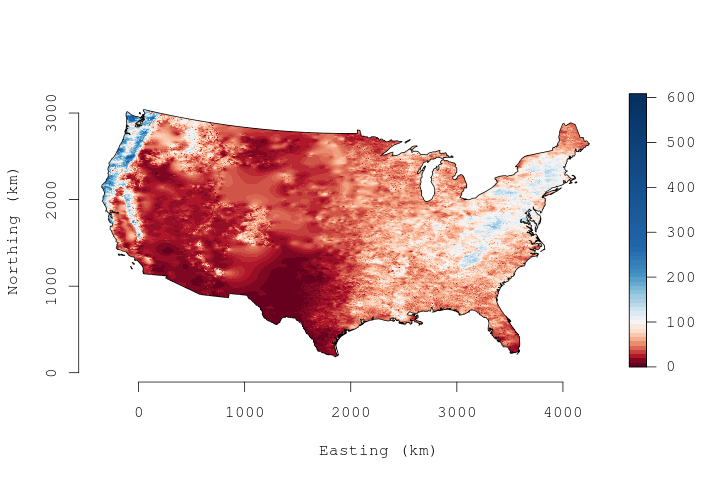
\includegraphics[width=5cm]{../figures/fitted-biomass.png}\label{bio-fitted}}\\  \vskip-2.5mm
\subfloat[$\beta_0(s)$]{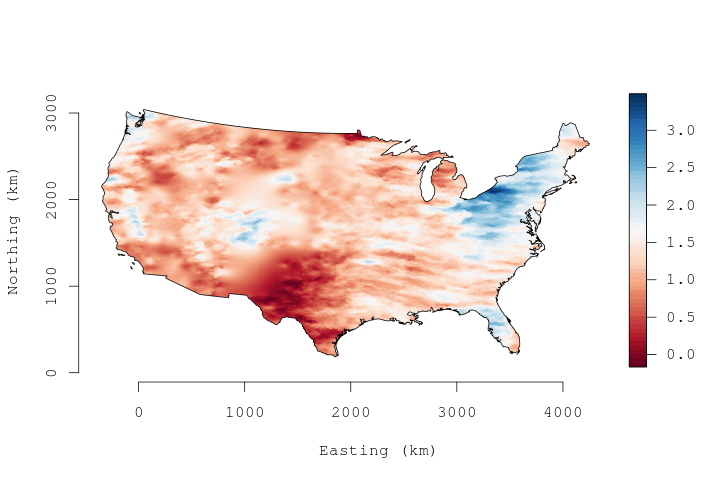
\includegraphics[width=5cm]{../figures/svc-beta0.png}\label{bio-coefs-b0}}
\subfloat[$\beta_{NDVI}(s)$]{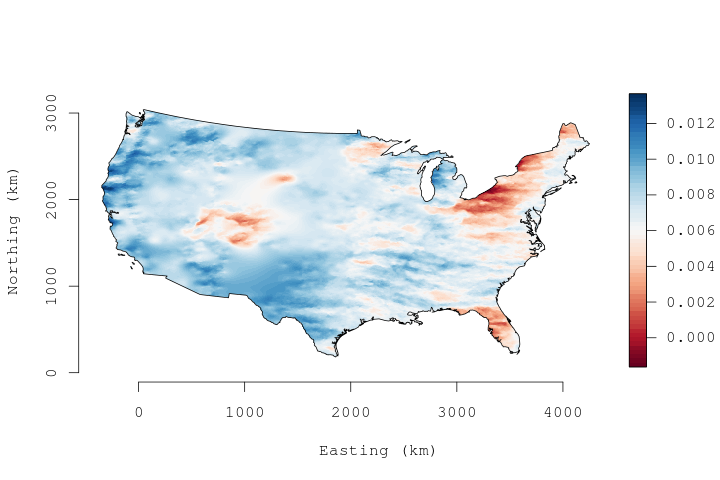
\includegraphics[width=5cm]{../figures/svc-beta1.png}\label{bio-coefs-b1}}\\
\end{center}
\label{fig:bio-coefs}
\end{figure}
\end{frame}

\begin{frame}{Reducing parameter dimensionality}
	\begin{itemize}
		\item The Gibbs sampler algorithm for the NNGP updates $w(s_1), w(s_2), \ldots, w(s_n)$ sequentially
		\item Dimension of the MCMC for this \alert{sequential} algorithm is \red{$O(n)$}
		\item If the number of data locations $n$ is very large, this \blue{high-dimensional} MCMC can converge slowly
		\item Although each iteration for the NNGP model will be very fast, \red{many more MCMC iterations} may be required
	\end{itemize}
\end{frame}

\begin{frame}{Collapsed NNGP}
	\begin{itemize}
		\item Same model: 
		\begin{align*}
		y(s) &= x(s)'\beta + w(s) + \eps(s)\\
		w(s) &\sim NNGP(0,C(\cdot,\cdot \given \theta))\\
		\eps(s) &\iid N(0,\tau^2)
		\end{align*}
		\item Vector form $y \sim N(X\beta + w, \tau^2 I); w \sim N(0, \tilde C(\theta))$
		\item \alert{Collapsed model:} \blue{Marginalizing} out $w$, we have $y \sim N(X\beta, \tau^2 I + \tilde C (\theta))$
	\end{itemize}
\end{frame}

\begin{frame}{Collapsed NNGP}
	\begin{alertblock}{Model}{$y \sim N(X\beta, \tau^2 I + \tilde C (\theta))$}
	\end{alertblock}
\begin{itemize}
	\item Only involves few parameters $\beta$, $\taus$ and $\theta=(\sigs, \phi)'$
	\item Drastically \red{reduces} the MCMC dimensionality
	\item Gibbs sampler updates are based on sparse linear systems using $\tilde C^{-1}$
	\item \green{Improved} MCMC convergence
	\item Can \blue{recover} posterior distribution of $w \given y$
	\item Complexity of the algorithm depends on the design of the data locations and is \red{not guaranteed to be $O(n)$}
\end{itemize}
\end{frame}

\begin{frame}{Response NNGP}
	\begin{itemize}
		\item $w(s) \sim GP(0, C(\cdot, \cdot \given \theta)) \Rightarrow y(s) \sim GP(x(s)'\beta, \Sigma(\cdot,\cdot \given \taus, \theta))$ 
		\item $\Sigma (s_i, s_j) = C( s_i , s_j \given \theta) + \taus \; \delta(s_i =s_j)$ ($\delta$ is Kronecker delta)
		\item We can directly derive the NNGP covariance function corresponding to $\Sigma(\cdot,\cdot)$
		\item $\tilde \Sigma$ is the NNGP covariance matrix for the $n$ locations
		\item \alert{Response model:} $y \sim N(X\beta, \tilde \Sigma)$
		\item Storage and computations are guaranteed to be $O(n)$
		\item Low dimensional MCMC  $\Rightarrow$ Improved convergence
		\item \red{Cannot} coherently recover $w \given y$
		\end{itemize}
\end{frame}

\begin{frame}{Comparison of NNGP models}
	\begin{table}[]
	\centering
		\begin{tabular}{c|c|c|c}
		&	Latent & Collapsed  & Response\\ \hline
$O(n)$ time & \green{Yes} &  \red{No} &  \green{Yes}  \\ \hline
Recovery of $w \given y$ & \green{Yes} & \green{Yes} & \red{No} \\ \hline
Parameter dimensionality & \red{High} & \green{Low} & \green{Low} 
		\end{tabular}
\end{table}
\end{frame}

\begin{frame}{Comparison of NNGP models}
\begin{center}\setcounter{subfigure}{0}% Reset subfigure counter
\begin{figure}[t!]
  \centering%trim={<left> <lower> <right> <upper>}
%  \subfloat{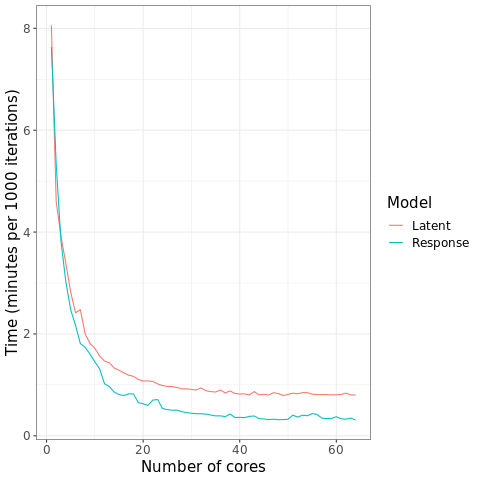
\includegraphics[trim=0cm 0cm 0cm 0cm,clip,width=5cm]{../figures/cpu_runtime.png}\label{cpuTiming}}
%  \subfloat{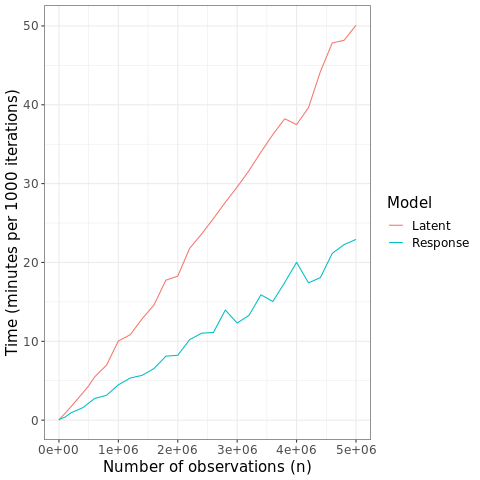
\includegraphics[trim=0cm 0cm 0cm 0cm,clip,width=5cm]{../figures/n_runtime.png}\label{nTiming}}
   \subfloat[b]{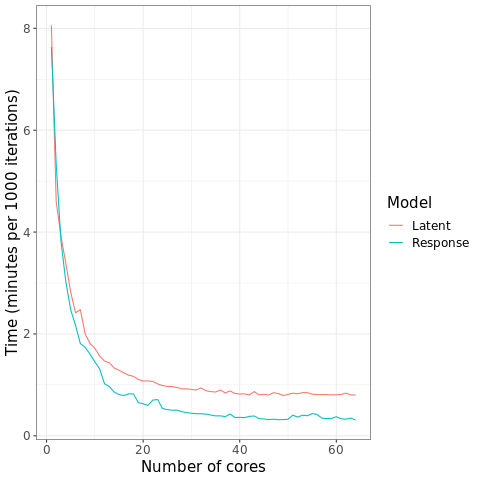
\includegraphics[trim=0cm 0cm 0cm 0cm,clip,width=5cm]{../figures/cpu_runtime.png}\label{cpuTiming}}  
   \subfloat[a]{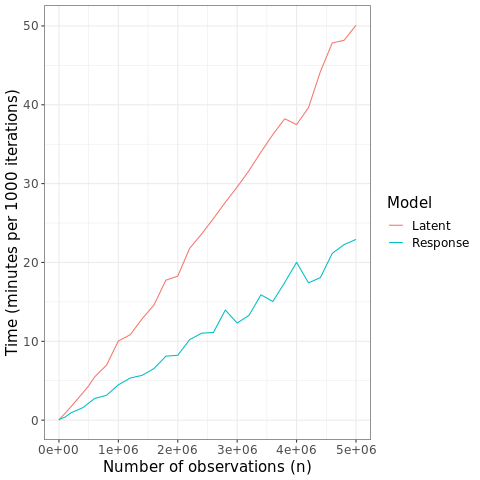
\includegraphics[trim=0cm 0cm 0cm 0cm,clip,width=5cm]{../figures/n_runtime.png}\label{nTiming}}
   \caption{\subref{cpuTiming} Runtime for 1000 MCMC iterations for
  $n=100000$ and different number of cores.  \subref{nTiming} Runtime for 1000
  MCMC iterations using 40 cores and $n$ from 1000 to 5
  million. Model type (latent and response) refers to different NNGP parameterizations.}
\end{figure}
\end{center}
\end{frame}

%\begin{frame}{Comparison of NNGP models}
%	\begin{figure}
%		\begin{center}
%			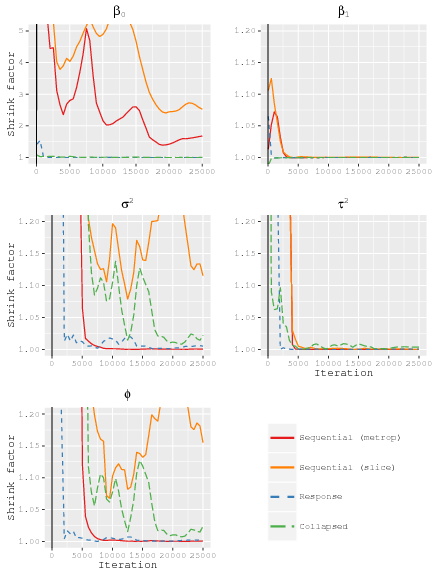
\includegraphics[scale=0.3]{../figures/syn-large-m15-gr.png}
%		\end{center}	
%		\caption{MCMC convergence diagnostics using Gelman-Rubin shrink factor for different NNGP models for a simulated dataset}
%	\end{figure}
%\end{frame}

\begin{frame}{Summary of Nearest Neighbor Gaussian Processes}
\begin{itemize}
\item \blue{Sparsity} inducing Gaussian process
\item Constructed from sparse Cholesky factors based on $m$ nearest neighbors
\item \red{Scalability:} Storage, inverse and determinant of NNGP covariance matrix are all $O(n)$
\item \blue{Proper Gaussian process}, allows for inference using hierarchical spatial models and predictions at \red{arbitrary spatial resolution}
\item Closely approximates full GP inference, does not oversmooth like low rank models
\item Extension to \blue{multivariate NNGP}
\item Collapsed and response NNGP models with improved MCMC convergence
\item \red{spNNGP package in R} for analyzing large spatial data using NNGP models
\end{itemize}
\end{frame}

\end{document}
